\documentclass[a4paper]{article}
\usepackage{float}
\usepackage[spanish,es-tabla]{babel}
\usepackage[T1]{fontenc}
\usepackage[spanish]{babel}
\usepackage{graphicx} 
\usepackage[utf8]{inputenc}
\usepackage{amsmath}
\usepackage{longtable}
\usepackage{graphicx}
\usepackage[colorinlistoftodos]{todonotes}
\usepackage[letterpaper,top=2.5cm,bottom=2.5cm,left=2cm,right=2cm,marginparwidth=2.5cm]{geometry}
\renewcommand{\baselinestretch}{1.25}


\title{Informe Física 5}
\author{Danny Córdova, Edwin Dávila}
\date{21 de Marzo del 2023}



\begin{document}

\maketitle

\section{Introducción}

En la presente práctica se estudió la cinemática de rotación. Este tipo de movimiento es uno de los más importantes en física debido a que introduce uno de los conceptos que está presente en muchos fenómenos físicos: el oscilador armónico. En la práctica se mide el tiempo en el que un obturador recorre una distancia angular de $\pi$ en un movimiento uniformemente acelerado por una masa. El objetivo general del experimento es deducir una ecuación en función del tiempo que mida el desplazamiento angular y la velocidad angular.

\section{Metodología experimental}

Las unidades usadas en este experimento son las del SI. Las incertidumbres de los instrumentos de medida son:

\begin{table}[H]
    \centering
    \begin{tabular}{|c|c|}
    \hline
        Calibrador Vernier & $\pm0,02 mm$ \\ \hline
        Regla  & $\pm 1 mm$ \\ \hline
        Cronómetro digital  & $\pm 0,01 ms$ \\ \hline
    \end{tabular}
    \caption{Incertidumbre de los instrumentos de medida}
    \label{Incertidumbre de los instrumentos de medida}
\end{table}

Cada medición del movimiento iba desde $\pi$ hasta $10\pi$, en total se hicieron 20 mediciones para el experimento. 

Las variables directas que se miden en este experimento son:
\begin{enumerate}
  \item Diámetro de la base (d).
  \item Tiempo de obturación (t).
  \item Ancho del obturador (x).
\end{enumerate}

Las variables indirectas que se calculan a partir de la información obtenida son:
\begin{enumerate}
  \item Velocidad angular ($\omega$).
  \item Aceleración angular ($\alpha$).
\end{enumerate}

Las fórmulas usadas en este experimento son:
\begin{equation}
    \mu= \frac{\displaystyle\sum_{i=1}^{n} x_i}{n}
\end{equation}
donde $\mu$ es la media o promedio del conjunto $x_i$ y n el número de elementos del conjunto $x_i$.

\begin{equation}
   v=\frac{\Delta d}{\Delta t}
\end{equation}
donde v es la velocidad tangencial, $\Delta d$  es la variación el ancho del obturador y $\Delta$t la variación del tiempo.

\begin{equation}
    \omega=\frac{v}{R}
\end{equation}
donde $\omega$ es la velocidad angular y R el radio de la base.

\begin{equation}
    y=mx+b
\end{equation}
esta fórmula representa la ecuación de una recta y sirve para hacer la regresión lineal. Aquí x es la variable independiente y y la variable dependiente. 

\begin{equation}
   m=\frac{\sum x_i*y_i-\frac{1}{n}\sum x_i \sum y_i}{\sum x_i^2-\frac{1}{n}(\sum x_i)^2} 
\end{equation}
donde m es la pendiente de la regresión lineal y n es el número de datos.

\begin{equation}
    b=\frac{\sum y_i}{n}-m\frac{\sum x_i}{n}
\end{equation}
donde b es el corte en el eje y de la regresión lineal.

\begin{equation}
    \int_{0}^{t} \alpha (t)dt= \omega(t)=\omega_0+\alpha t
\end{equation}
donde $\alpha$ es la aceleración angular, $\omega$ la velocidad angular, $\omega_0$ la velocidad angular inicial y t el tiempo. Esta fórmula solo se puede usar para un $\alpha$ constante. 

\begin{equation}
    \int_{0}^{t} \omega(t)dt= \theta (t) = \theta_0+\omega_0 t+\frac{\alpha t^2}{2}
\end{equation}
donde $\omega$ es la velocidad angular. 

\begin{equation}
    \omega_f^2=\omega_o^2+2\alpha \Delta \theta
\end{equation}
donde $\omega_f^2$ es la velocidad angular final y $\Delta \theta$ la variación en el ángulo. 

\section{Resultados y observaciones}
Luego de tomar los tiempos de obturación cada $\pi$ (ver Anexos), se obtienen los promedios de tiempo de obturación usando la fórmula (1).

\begin{table}[!ht]
    \centering
    \begin{tabular}{|c|c|c|c|c|c|c|c|c|c|}
    \hline
        $\pi$ & 2$\pi$ & 3$\pi$ & 4$\pi$ & 5$\pi$ & 6$\pi$ & 7$\pi$ & 8$\pi$ & 9$\pi$ & 10$\pi$  \\ \hline
        42,829  & 30,109  & 25,0135  & 21,7435  & 19,497  & 17,8135  & 16,411  & 15,3225  & 14,433  & 13,971  \\ \hline
    \end{tabular}
    \caption{Tiempo de obturación promedio (en ms) cada $\pi$}
\end{table}

A partir de estos tiempos se calcula $\omega$ considerando el radio desde el centro del disco hasta el sensor y el ancho del obturador usando las fórmulas (2) y (3).

\begin{table}[!ht]
    \centering
    \begin{tabular}{|c|c|c|c|c|c|c|c|c|c|}
    \hline
       $\pi$ & 2$\pi$ & 3$\pi$ & 4$\pi$ & 5$\pi$ & 6$\pi$ & 7$\pi$ & 8$\pi$ & 9$\pi$ & 10$\pi$  \\ \hline
        1,6900  & 2,4039  & 2,8936  & 3,3288  & 3,7123  & 4,0632  & 4,4104  & 4,7237  & 5,0149  & 5,1807  \\ \hline
    \end{tabular}
    \caption{Velocidad angular (en rad/s) cada $\pi$}
\end{table}

A partir de estos datos se obtiene la siguiente gráfica: 
\begin{figure} [H]
    \centering
    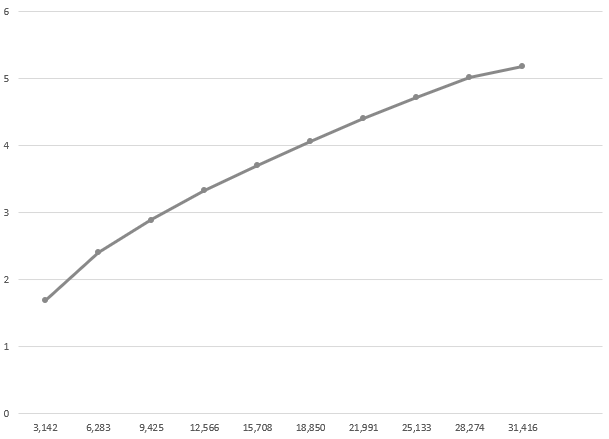
\includegraphics[width=0.6 \textwidth]{VangvsDang.png}
    \caption{Velocidad angular (eje y) en función del desplazamiento angular (eje x)}
    \end{figure}

Considerando ahora la velocidad angular al cuadrado $\omega^2$: 

\begin{table}[!ht]
    \centering
    \begin{tabular}{|c|c|c|c|c|c|c|c|c|c|}
    \hline
        $\pi$ & 2$\pi$ & 3$\pi$ & 4$\pi$ & 5$\pi$ & 6$\pi$ & 7$\pi$ & 8$\pi$ & 9$\pi$ & 10$\pi$  \\ \hline
        2,8560  & 5,7788  & 8,3730  & 11,0809  & 13,7815  & 16,5095  & 19,4519  & 22,3138  & 25,1489  & 26,8397  \\ \hline
    \end{tabular}
    \caption{Velocidad angular al cuadrado (en rad/$s^2$) en función del desplazamiento angular}
\end{table}

A partir de estos datos generamos la siguiente gráfica: 
\begin{figure} [H]
    \centering
    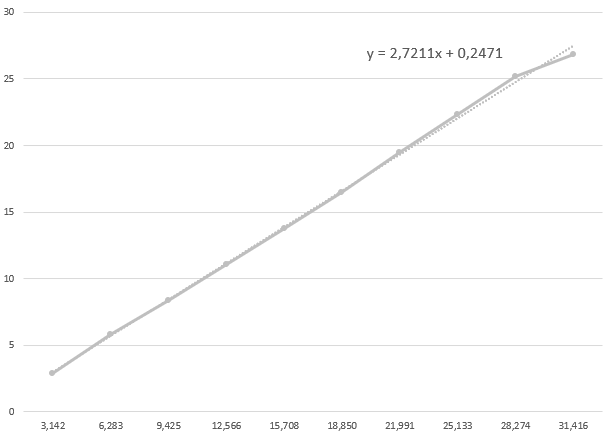
\includegraphics[width=0.6 \textwidth]{Vang^2vsDang.png}
    \caption{Velocidad angular al cuadrado (eje y) en función del desplazamiento angular (eje x)}
    \end{figure}
    
Haciendo uso de las fórmulas (4), (5), (6), se tiene la siguiente función lineal:

\[ y= 0,2471 + 2,7211x\]

Ahora, esta función toma los valores de $\pi$ como si fueran la unidad, entonces la ecuación de la recta tomando esto en cuenta es:

\[ y= 0.86615x+0.079654\]

Esto representa la ecuación (9). Donde 0.07965$\frac{rad}{s}$ es nuestro $\omega_o^2$ y 0.86615$\frac{rad}{s^2}$ es 2$\alpha$.

A partir de estos datos y haciendo uso de las fórmulas (7) y (8) se tiene:

\[\omega(t)=0.282230+0.433075t\]
\[\theta(t)=0.282230t+\frac{0.433075 t^2}{2}\]

Haciendo uso de la herramienta digital GeoGebra, la gráfica de las funciones es la siguiente:

\begin{figure} [H]
    \centering
    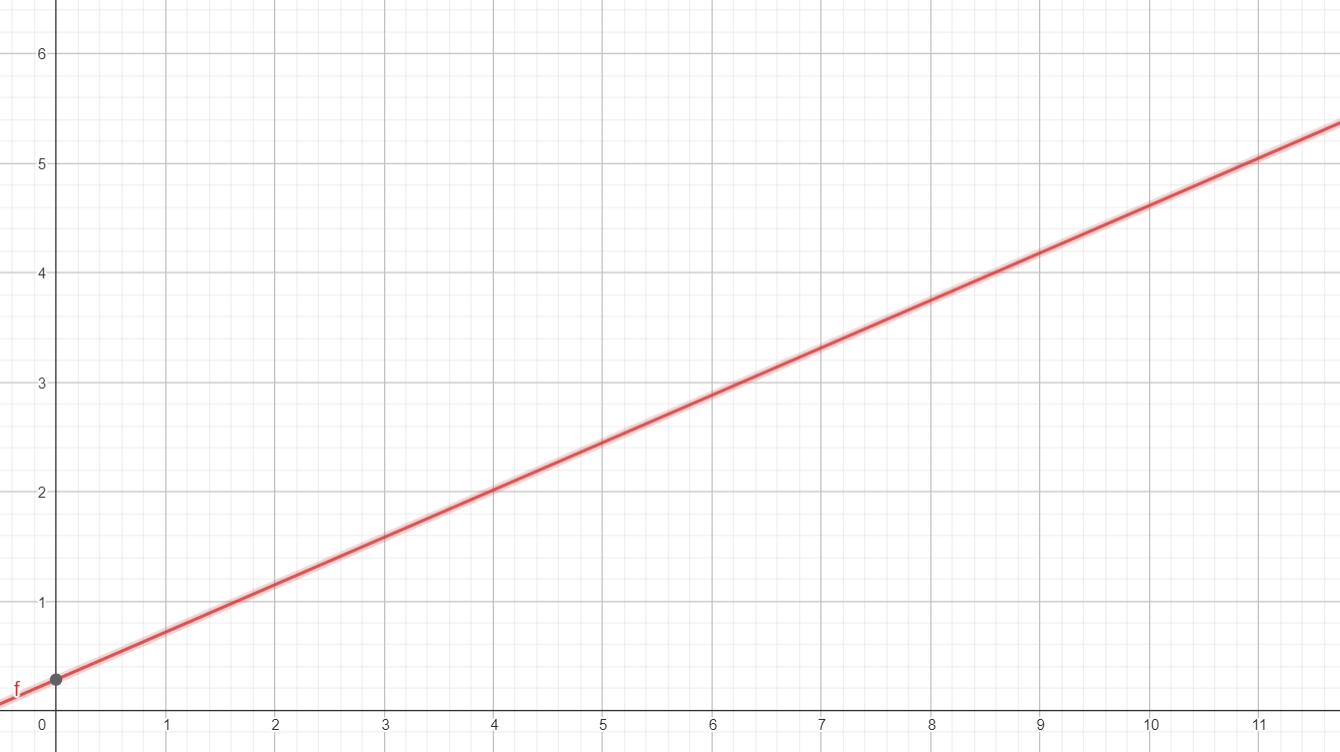
\includegraphics[width=0.6 \textwidth]{omega(t).png}
    \caption{Velocidad angular en función del tiempo $\omega (t)$}
    \label{omega}
\end{figure}

\begin{figure} [H]
    \centering
    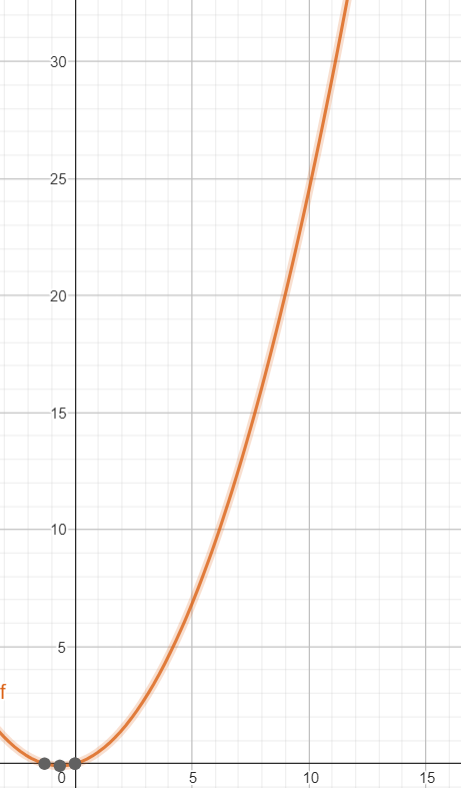
\includegraphics[width=9cm, height=14cm]{theta(t).png}
    \caption{Desplazamiento angular en función del tiempo $\omega (t)$}
    \label{theta}
\end{figure}

\section{Conclusiones}
En esta práctica se pudo comprobar que se puede modelar matemáticamente mediante la cinemática el movimiento rotacional. El modelo no describe con exactitud al movimiento en la realidad porque en el experimento no se toma en cuenta a fuerzas no conservativas como fricción con el aire y fricción con la base. Sin embargo, el objetivo general de la práctica se cumplió satisfactoriamente y se pudo tener las ecuaciones para la velocidad angular y el desplazamiento angular.

\section{Anexos}

\begin{table}[!ht]
    \centering
    \begin{tabular}{|c|c|c|c|c|c|c|c|c|c|c|}
    \hline
         & $\pi$ & 2$\pi$ & 3$\pi$ & 4$\pi$ & 5$\pi$ & 6$\pi$ & 7$\pi$ & 8$\pi$ & 9$\pi$ & 10$\pi$ \\ \hline
        1 & 42,98 & 30,24 & 24,76 & 21,47 & 19,37 & 17,76 & 16,33 & 15,25 & 14,34 & 14,11
\\ \hline
        2 & 43,59 & 30,82 & 24,98 & 21,64 & 19,25 & 17,54 & 16,18 & 15,16 & 14,26 & 13,99
\\ \hline
        3 & 42,85 & 30,52 & 24,87 & 21,62 & 19,17 & 17,49 & 16,1 & 15,1 & 14,18 & 13,98
\\ \hline
        4 & 42,76 & 30,23 & 24,73 & 21,52 & 19,16 & 17,5 & 16,15 & 15,12 & 14,22 & 13,99
\\ \hline
        5 & 42,27 & 30,06 & 24,82 & 21,62 & 19,33 & 17,65 & 16,25 & 15,22 & 14,35 & 14,12
\\ \hline
        6 & 43,18 & 30,6 & 24,95 & 21,58 & 19,16 & 17,47 & 16,1 & 15,09 & 14,18 & 13,55
\\ \hline
        7 & 42,7 & 30,18 & 25,07 & 21,84 & 19,44 & 17,73 & 16,34 & 15,3 & 14,39 & 13,8
\\ \hline
        8 & 43,34 & 30,67 & 25,49 & 22,07 & 19,78 & 18,07 & 16,67 & 15,53 & 14,65 & 14,29
\\ \hline
        9 & 42,27 & 29,89 & 24,98 & 21,75 & 19,93 & 18,36 & 16,85 & 15,68 & 14,77 & 14,56
\\ \hline
        10 & 42,64 & 29,82 & 25,17 & 21,93 & 19,79 & 18,17 & 16,69 & 15,57 & 14,67 & 14,19
\\ \hline
        11 & 42,86 & 30,1 & 24,73 & 21,43 & 19,24 & 17,6 & 16,23 & 15,19 & 14,33 & 13,85
\\ \hline
        12 & 42,71 & 29,8 & 24,46 & 21,52 & 19,17 & 17,49 & 16,15 & 15,1 & 14,25 & 13,67
\\ \hline
        13 & 42,62 & 30,04 & 25,3 & 21,99 & 19,82 & 18,1 & 16,68 & 15,53 & 14,64 & 14,17
\\ \hline
        14 & 43,61 & 29,99 & 25,53 & 22,13 & 20,04 & 18,32 & 16,87 & 15,65 & 14,68 & 14,29
\\ \hline
        15 & 42,66 & 29,72 & 25,18 & 21,83 & 19,84 & 18,19 & 16,73 & 15,55 & 14,68 & 14,19
\\ \hline
        16 & 42,89 & 30,11 & 25,26 & 22,09 & 19,48 & 17,65 & 16,35 & 15,31 & 14,44 & 13,73
\\ \hline
        17 & 42,77 & 29,8 & 25,06 & 21,77 & 19,44 & 17,7 & 16,32 & 15,21 & 14,37 & 13,67
\\ \hline
        18 & 42,74 & 29,85 & 24,94 & 21,66 & 19,37 & 17,64 & 16,29 & 15,17 & 14,33 & 13,67
\\ \hline
        19 & 42,43 & 29,81 & 24,85 & 21,64 & 19,44 & 17,76 & 16,34 & 15,25 & 14,38 & 13,72
\\ \hline
        20  & 42,71  & 29,93  & 25,14  & 21,77  & 19,72  & 18,08  & 16,6  & 15,47  & 14,55  & 13,88
\\ \hline
    \end{tabular}
    \caption{Tiempos de obturación cada $\pi$}
\end{table}

\end{document}